\tikzset{every picture/.style={line width=0.75pt}} %set default line width to 0.75pt        

\begin{tikzpicture}[x=0.75pt,y=0.75pt,yscale=-1,xscale=1]
%uncomment if require: \path (0,178); %set diagram left start at 0, and has height of 178

%Straight Lines [id:da4174001315479594] 
\draw  [->]  (165,50) -- (325,50) ;
%Straight Lines [id:da7329900163828524] 
\draw  [<-]  (165,90) -- (325,90) ;
%Straight Lines [id:da23828684375566445] 
\draw  [->]  (165,130) -- (325,130) ;
%Straight Lines [id:da16375144538818653] 
\draw  [line width=0.5]  (38,19) -- (122,19) ;
%Straight Lines [id:da8683098306105947] 
\draw  [line width=0.5]  (352,19) -- (428,19) ;

% Text Node
\draw (80,10) node    {$P( \alpha _{1} \in \mathbb{H}_{1} ,\psi )$};
% Text Node
\draw (391,10) node    {$V( u\in \mathbb{H}_{2} ,\psi )$};
% Text Node
\draw (245,86.6) node [anchor=south] [inner sep=0.75pt]    {$c\in \mathbb{Z}$};
% Text Node
\draw (245,126.6) node [anchor=south] [inner sep=0.75pt]    {$\alpha _{\mathrm{z}} \in \mathbb{H}_{1}$};
% Text Node
\draw (80,30) node    {$\alpha _{\mathrm{t}}\overset{\mathrm{R}}{\leftarrow }\mathbb{H}_{1} ,\ u_{\mathrm{t}}\leftarrow \psi ( \alpha _{\mathrm{t}})$};
% Text Node
\draw (391,70) node    {$c\overset{\mathrm{R}}{\leftarrow }\mathcal{C}$};
% Text Node
\draw (80,110) node    {$x_{\mathrm{z}}\leftarrow \alpha _{\mathrm{t}} +\alpha \cdot c\in \mathbb{H}_{1}$};
% Text Node
\draw (245,46.6) node [anchor=south] [inner sep=0.75pt]    {$u_{\mathrm{t}} \in \mathbb{H}_{2}$};
% Text Node
\draw (391,150) node    {$\psi ( \alpha _{\mathrm{z}})\overset{?}{=} u_{\mathrm{t}} \cdot u^{c}$};


\end{tikzpicture}